The efficacy of the selected metamodels has been tested on 
a pair of pseudo-engineering optimization problems, where the exact 
PSM is cheap in terms of computational cost. The study now focuses 
on performing a comparison between MAEAs, i.e. both the methods and 
the metamodels will be evaluated, and plain EAs when implemented in 
the shape optimization of a 2D airfoil. The parameters of the 
optimization are computed by solving the steady-state 
Reynolds-Averaged Navier-Stokes (RANS) equations for compressible 
flows via the use of the one-equation turbulence model 
Spalart-Allmaras \cite{Spalart Allmaras}. Consequently in this 
case, the exact PSM model is a CFD model, which is solved using 
PUMA software (Parallel solver, for Unstructured grids, for 
Multi-blade row computations, including Adjoint) \cite{PUMA} 
developed by the PCOpt/NTUA. The entirety of the CFD evaluations 
are performed on Nvidia Tesla K40 12 GB GPUs, using a GPU-enabled 
variant \cite{PUMA_GPU} of PUMA programmed in CUDA.
\vfill


\section{Mesh and parametrization}

The accuracy and the computational cost of CFD evaluations highly
depends on the type and quality of the airfoil mesh. There are 
three types of grids regarding their structure; structured, 
unstructured and hybrid. 
%The former are constructed based on the 
%idea that the nodes of the grid must be connected sequentially, in 
%such a way that each node can be represented computationally by the 
%indexes $(i,j) \!\in \!\mathbb{Z}^{+2}$ in the system memory. 
%Consequently, all adjacent nodes can be easily found by searching 
%entries $+1, -1$ in the system memory, e.g. $(i+1,j)$. Structured 
%grid solvers are usually faster in terms of convergence, however, 
%hey lack in accuracy. In unstructured grids, on the other hand, 
%the nodes are connected forming tetrahedra, pyramids, prisms or 
%hexahedra, where each cell is denoted by single pointer $i \!\in 
%\!\mathbb{Z}^{+}$ in system memory. 
Due to the formation of 
unstructured grids, unstructured solvers are commonly slower then 
structured ones. However, the constant increase of computational 
power, along with the high adaptability to any geometry and the 
fast construction time, lead to the widespread use of unstructured 
grids in CFD applications. In this diploma thesis, a structured 
C-type grid is generated for the purpose of the study, as seen in 
figure \ref{fig:mesh}, which is handled by PUMA as a 
hybrid grid of tetrahedral cells. C-type grids are preferred due to 
their shape that matches the trailing edge curvature, thus 
effectively capturing the wake in viscous flows.

The second parameter that affects the accuracy and the 
computational cost of CFD evaluations is the quality of the mesh.
The higher the resolution of the mesh, the greater the accuracy of 
the outcome. The construction of a high-resolution mesh would, 
however, severely increase the number of nodes where the RANS need 
to be solved. In a steady-state compressible flow, turbulence is 
developed near the walls, i.e. in the viscous sublayer, and in the 
wake of the airfoil, where a finer mesh is needed in order to 
account for the small fluctuations in the values of flow 
components. Consequently, a mesh of ranging resolution is 
implemented; coarse in the far field and fine near the walls and 
in the wake of the airfoil. 

\newpage
%------------------------------------------------------------------

\begin{figure}[h!]
\centering
	\begin{subfigure}[b]{0.49\textwidth}
	\centering
	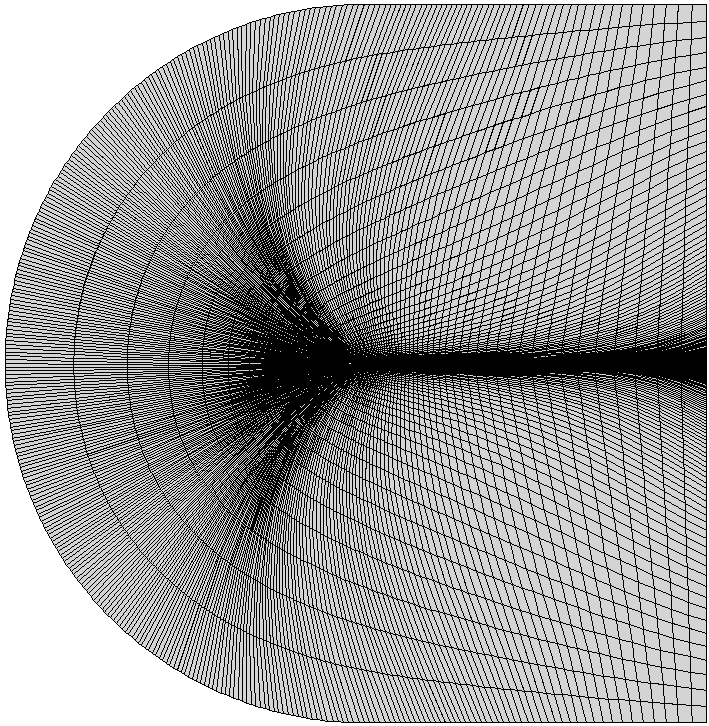
\includegraphics[width=\textwidth, height=0.8\textwidth, 
	scale=1]{mesh.png}   
	\end{subfigure}
	\hfill
	\begin{subfigure}[b]{0.49\textwidth}
	\centering
	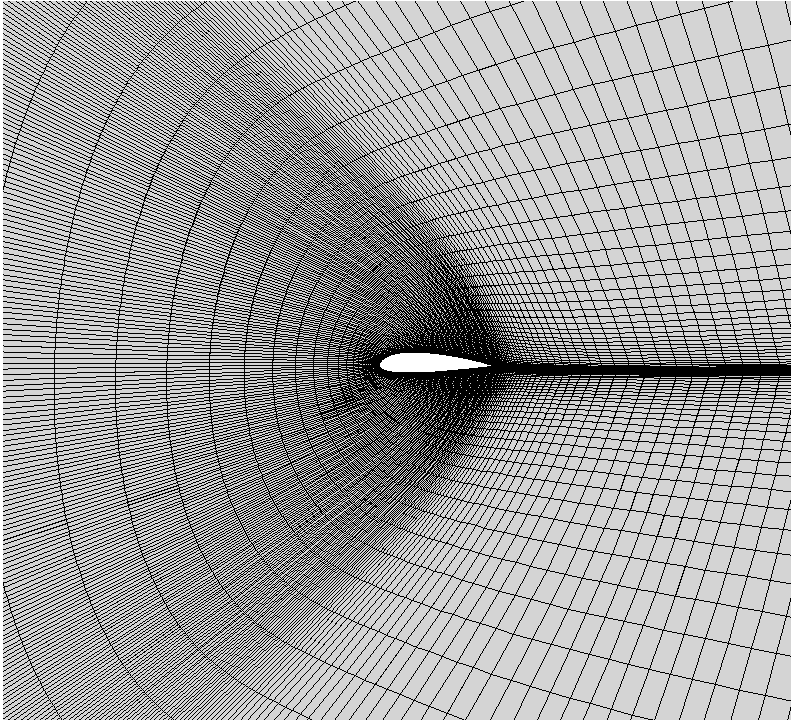
\includegraphics[width=\textwidth, height=0.8\textwidth, 
	scale=1]{mesh2.png}   
	\end{subfigure}
\caption{2D C-type structured mesh} 
\label{fig:mesh}
\end{figure}

%Based on this principle, a pseudo-3D computational mesh can be 
%defined by four patches, each one of which can be represented by a 
%2D plane. The first patch contains the grid nodes in the far-field 
%flow, while the first off the wall nodes are placed at $y^{+} = 1$ 
%and contained at a separate patch, where $y^{+}$ is the 
%dimensionless wall normal distance. The remaining nodes of the 
%front 2D plane of the airfoil are contained in the next patch, 
%which is subsequently replicated and shifted in the $z$ direction
%in order to construct a pseudo-3D mesh. The flow properties are 
%only computed in the front slice of the airfoil and are then copied 
%to the back slice. This pseudo-3D design is used to reduce the 
flow 
%equations in 2 dimensions, i.e. $x$ and $y$.

The optimization process aims at yielding the airfoil shape that 
minimizes or maximizes the flow properties, e.g. $C_{L}$, $C_{D}$, 
under certain imposed flow conditions and constraints. The 
modification of the airfoil shape is performed via univariate Non 
Uniform Rational B-Splines (NURBS). The used NURBS are built via 
the interpolation of 15 control points in 2D space and produce the
curves of the airfoil. Subsequently, the nodes contained in the 
front patch of the grid are shifted in order to adapt to the new 
airfoil shape using the spring analogy method, according to which 
the grid is modelled as net of linear springs with elasticity 
proportional to the inverse of mesh edge length. The control points 
of the volumetric NURBS are displaced in the $y$ direction during 
the optimization and the airfoil shape is modified accordingly.
Consequently, the 13 $y$ coordinates of the control points are set 
as the design variables of the optimization; the $y$ coordinates 
of the control points corresponding to the leading edge and 
trailing edge points are kept fixed, as depicted in figure 
\ref{fig:NURBS_airfoil}.

\begin{figure}[h!]
\centering
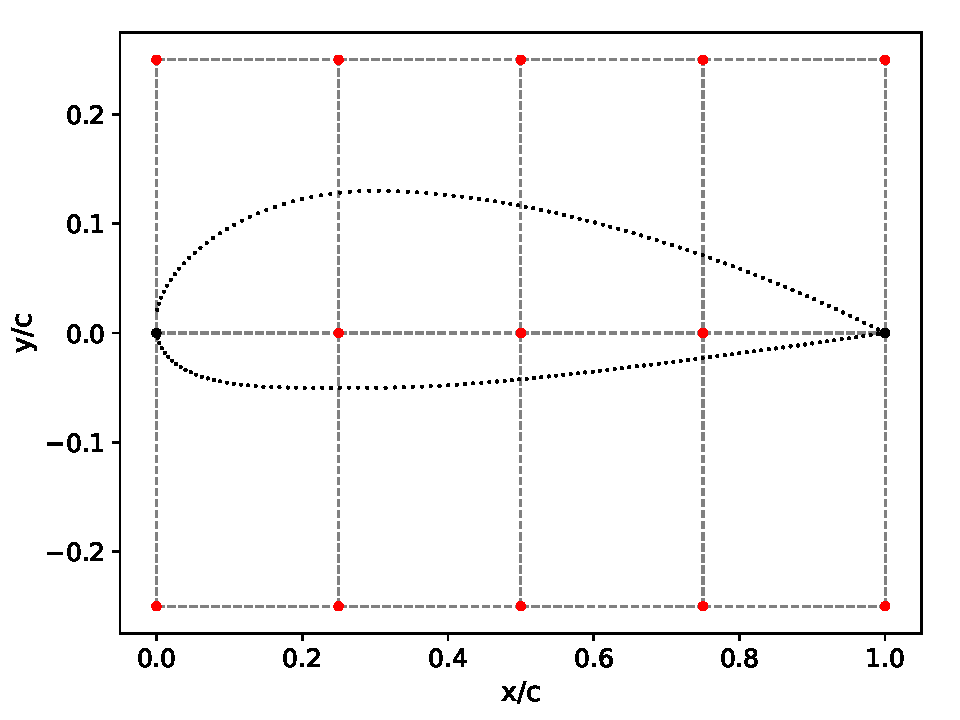
\includegraphics[width=0.5\textwidth, height=0.35\textwidth]
{NURBS.pdf}   
\caption{Design of NACA 4318. Parametrization of the baseline 
airfoil geometry using volumetric NURBS with control points that 
have one (red) or none (black) degree of freedom.} 
\label{fig:NURBS_airfoil}
\end{figure}

\newpage
%---------------------------------------------------------------


\section{RANS flow equations}
%The Navier-Stokes continuity, momentum and energy partial 
%differential equations for steady-state compressible flows are 
%given by\footnote{For brevity, the Einstein summation convention 
%for repeated indices is applied in all flow-related equations}:
%\begin{equation}\label{compressible NS}
%\begin{split}
%& \dfrac{\partial ρ}{\partial t} + \dfrac{\partial }{\partial 
%x_{j}}(ρu_{j}) = 0
%\\ &
%\dfrac{\partial }{\partial t} (ρu_{i}) + \dfrac{\partial }{\partial 
%x_{j}}(ρu_{i}u_{j} + pδ_{ij} -τ_{ij}) = 0, 
%\hspace{8mm} \text{for} \hspace{2mm} i =1,2
%\\ &
%\dfrac{\partial }{\partial t} (ρE) + \dfrac{\partial }{\partial 
%x_{j}}(ρu_{j}E + u_{j}p - q_{j} - u_{i}τ_{ij}) = 0 
%\end{split}
%\end{equation}
%\\[-2mm]
%where $δ_{ij}$ is the Kroenecker delta, $ρ$ the density of the 
%fluid, in this case air, $u_{i}$ the flow field velocity, $E$ 
%denotes the energy per unit mass, which when multiplied by the 
%density $ρ$ produces the the total energy per unit volume, denoted 
%by $E_{t}$ and given by:
%\begin{equation}
%E_{t} = ρE = \dfrac{p}{γ-1} + \dfrac{1}{2}u_{i}u_{i}
%\end{equation}
%\\[-1mm]
%where $γ$ is the gas specific heat ratio, which for air is equal to 
%$γ =$ \scalebox{0.85}{ %
%$\dfrac{C_{p}}{C_{v}} $} $= 1.4$. The constant parameters $C_{p}$,
%$C_{\mathrm{v}}$ denote the specific heat under constant pressure 
%and constant volume, respectively. The term $τ_{ij}$ that appears 
%in momentum and energy equation, denotes the viscous stress tensor:
%\begin{equation}
%τ_{ij} = \dfrac{μ}{Re} \left( \dfrac{\partial u_{i}}{\partial 
%x_{j}} + \dfrac{\partial u_{j}}{\partial x_{i}} \right)
%\end{equation}

%\newpage
%%-----------------------------------------------------------------

%In order to decrease the 
%computational cost of solving the Navier-Stokes equations in 
%turbulent flows, the aforementioned equations are restated and 
%solved w.r.t. the mean flow quantities. Following the Reynolds 
%decomposition, the flow field can be expressed as: 
%\begin{equation}
%u_{i}(x, t) = \overline{u}_{i}(x) + u_{i}'(x, t)
%\end{equation}   
%\\[-2mm]
%where $\overline{u}_{i}$ is the time-averaged or mean component 
%calculated as such:
%\begin{equation}
%\overline{u}_{i}(x) = \dfrac{1}{T_{p}} \int_{t}^{t+T_{p}} 
%u_{i}(x, t) dt
%\end{equation}
%\\[-2mm]
%where $u_{i}'(x, t)$ are the flow field fluctuations, which are 
%equal to zero when time-averaged. In compressible flows, the 
%Reynolds decomposition of flow quantities result in several terms 
%that need to be modelled due to density fluctuations. For this 
%reason, Favre or mass averaging is implemented, where the 
%respective Favre-averaged flow field is expressed as:
%\begin{equation}
%u_{i}(x, t) = \tilde{u}_{i}(x) + u_{i}''(x, t)
%\end{equation} 
%\\[-2mm]
%where $\tilde{u}_{i} =$ \scalebox{0.8}{%
%$\dfrac{\overline{ρu_{i}}}{\overline{ρ}}$}, where the overline 
indicates Reynolds averaging. If Favre averaging is 
applied to all flow quantities, then the continuity, momentum and 
energy RANS equations can be formulated as such\footnote{For 
brevity, the Einstein summation convention for repeated indices is 
applied in all flow-related equations}:
\begin{equation}
\begin{split}
& \dfrac{\partial \overline{ρ}}{\partial t} + \dfrac{\partial }
{\partial x_{j}}(\overline{ρ} \tilde{u}_{j}) = 0
\\ &
\dfrac{\partial }{\partial t} (\overline{ρ} \tilde{u}_{i}) + 
\dfrac{\partial }{\partial x_{j}}(\overline{ρ} \tilde{u}_{i}
\tilde{u}_{j} + \overline{p}δ_{ij} - \tilde{τ}_{ij}^{tot}) = 0, 
\hspace{8mm} \text{for} \hspace{2mm} i =1,2
\\ &
\dfrac{\partial }{\partial t} (\overline{ρ}\tilde{E}) + 
\dfrac{\partial}{\partial x_{j}}(\overline{ρ}\tilde{u}_{j}E + 
\tilde{u}_{j}\overline{p} - \tilde{q}_{j}^{tot} - \tilde{u}_{i} 
\tilde{τ}_{ij}^{tot}) = 0 
\end{split}
\end{equation}
\\
where Reynolds averaging is indicated by the overline. The RANS 
equations can be also written in conservative form:
\begin{equation}\label{conservative RANS}
\dfrac{\partial \vec{U}} {\partial t} + 
\dfrac{\partial \vec{f}_{j}^{inv}}{\partial x_{j}} -
\dfrac{\partial \vec{f}_{j}^{vis}}{\partial x_{j}} = 0
\end{equation}
\\[-1mm]
where in 2D flow $j = 1,2$ and $\vec{U} = [\overline{ρ}, 
\overline{ρ} \tilde{u}, \overline{ρ} \tilde{\mathrm{v}}, 
\overline{ρ}\tilde{Ε}]^T$ is the conservative flow variable vector 
with components the averaged terms in the continuity, 
momentum and energy Navier-Stokes equations for compressible flows. 
The inviscid and viscous fluxes denoted by $\vec{f}_{i}^{inv}$ and
$\vec{f}_{j}^{vis}$, respectively, and expressed as:

\begin{equation}
\vec{f}_{j}^{inv} = 
\begin{bmatrix}
\overline{ρ} \tilde{u}_{j} \\ 
\overline{ρ} \tilde{u}_{1}\tilde{u}_{j} + \overline{p}δ_{ij} \\ 
\overline{ρ} \tilde{u}_{2}\tilde{u}_{j} + \overline{p}δ_{ij} \\ 
\tilde{u}_{j} ( \tilde{E}_{t} + \overline{p} )
\end{bmatrix}
, \hspace{2mm}
\vec{f}_{j}^{vis} = 
\begin{bmatrix}
0 \\ 
\tilde{τ}_{1j}^{tot} \\ 
\tilde{τ}_{2j}^{tot} \\ 
\tilde{q}_{j}^{tot} + \tilde{u}_{i} \tilde{τ}_{ij}^{tot}
\end{bmatrix}
\end{equation}
\\[-2mm]
where:
\begin{equation}
\begin{split}
& \tilde{E}_{t} = \dfrac{\overline{p}}{γ-1} + \dfrac{1}{2} 
\left( \tilde{u}_{i}\tilde{u}_{i} +  
\dfrac{\overline{ρu_{i}''u_{i}''}}{\overline{p}} \right) 
\\[3mm] &
\tilde{τ}_{ij}^{tot} = \dfrac{μ + μ_{t}}{Re} \left( \dfrac{\partial 
\tilde{u}_{i}}{\partial x_{j}} + \dfrac{\partial \tilde{u}_{j}}
{\partial x_{i}} \right) 
-\dfrac{1}{3Re}δ_{ij}
\dfrac{\overline{ρu_{i}''u_{i}''}}{\overline{p}}
\\[2mm] &
\tilde{q}_{j}^{tot} = \dfrac{Cp}{Re} \left( \dfrac{μ}{Pr} + 
\dfrac{μ_{t}}{Pr_{t}} \right) \dfrac{\partial \tilde{T}_{s}}
{\partial x_{j}}
\end{split}
\end{equation}
\\
where $μ_{t}$ the turbulent or eddy viscosity and $Pr$, $Pr_{t}$ 
the Prandtl and the turbulent Prandtl number, respectively. 
The stress tensor depends on the molecular or dynamic viscosity of 
the fluid, denoted by $μ$, and the Reynolds number $Re$ given by:
\begin{equation}
Re = \dfrac{ρul}{μ}
\end{equation}

\newpage
%-----------------------------------------------------------------


where $l$ the characteristic length of the airfoil, which in this 
case is normalized using the chord length $c$, so $l \!\in 
\![0,1]$. The term $q_{j}$ that appears in energy equation denotes
the $j_{th}$ component of the heat flux and $\tilde{T}_{s}$ is the 
static temperature, which for an ideal gas is given by:
\begin{equation}
\tilde{T}_{s} = \dfrac{\overline{p}}{ρΡ_{g}}
\end{equation}
\\[-2mm]
where $R_{g}$ is the specific gas constant, which for air is 
$R_{g} = 287 \hspace{1mm} J/kgK$. The gas specific heat ratio is 
equal to $γ =$ \scalebox{0.85}{ %
$\dfrac{C_{p}}{C_{v}} $} $= 1.4$. The constant parameters $C_{p}$,
$C_{\mathrm{v}}$ denote the specific heat under constant pressure 
and constant volume, respectively. The term $τ_{ij}$ that appears 
in momentum and energy equation, denotes the viscous stress tensor.
%\begin{equation}
%q_{j} = \dfrac{μ}{Re} \dfrac{Cp}{Pr}
%\dfrac{\partial T_{s}}{\partial x_{j}}
%\end{equation}
%\\[-2mm]

The RANS steady-state equations are discretized using finite volume 
method and intergraded in pseudo-time and can be subsequently 
solved using a 3rd order Runge-Kutta scheme with residual 
smoothing, in this case flux Jacobian technique, developed by the 
Lab of Thermal Turbomachines (LTT), is used to 
smooth the residuals. The smoothing process requires the 
implementation of a linear algebra solver and, in this case, 
Gauss-Seidel method is applied. The process of calculating the RANS 
residuals is iterative and converges after the residuals have 
reached a user-defined value or a user-defined number of 
pseudo-time steps has been reached.

The no-penetration condition is applied, i.e. the normal component 
of the relative to the wall velocity is set to zero 
$\vec{\tilde{u}} \cdot \vec{n} = 0$ for stationary walls. The 
no-slip wall condition is applied in Spalart Allmaras transport 
equation and $\tilde{ν}$ is set to zero near the wall. The solid 
walls of the airfoil are subsequently modelled as adiabatic and the 
normal component of the relative to the wall heat flux is set to 
zero $\vec{\tilde{q}}_{j}^{tot} \cdot \vec{n} = 0$.
 

\newpage
%------------------------------------------------------------------


\section{Turbulence model} 
In order to improve the boundary layer prediction in the presence 
of adverse pressure gradients various turbulence models are 
employed. In this thesis, one-equation Spalart-Allmaras turbulence 
model is implemented, which is based on the observation that on a
flat plate in the log-law region of the boundary layer 
($y^{+} \!> \!30$) the profile of turbulence kinematic viscosity 
$ν_{t}$ with $y^{+}$ is linear, while in the viscous sublayer 
($y^{+} \!< \!5$) the profile is quartic. If however we assume a 
new variable $\tilde{ν}$, similar to $ν_{t}$, with linear profile
w.r.t. $y^{+}$ in the entirety of the sublayer region, then we can 
produce more stable results near the solid wall while 
simultaneously reducing the computational cost that arises from 
constructing a fine mesh near the solid wall. In order to account 
for any geometry and possible flow conditions, $\tilde{ν}$ is 
calculated by solving the modelled transport equation for 
compressible flows \cite{SA clarification}:
\begin{equation}\label{Spalart Allmaras}
\begin{split}
\dfrac{\partial}{\partial t}(ρ\tilde{ν}) + \dfrac{\partial}
{\partial x_{j}}(ρ\tilde{ν}u_{j}) = & 
\dfrac{ρ}{σ_{w}Re} \left[ \dfrac{\partial}{\partial x_{j}} \left( 
(\tilde{ν} + ν) \dfrac{\tilde{ν}}{\partial x_{j}} \right) 
+ c_{b2} \dfrac{\partial \tilde{ν}}{\partial x_{j}} 
\dfrac{\partial \tilde{ν}}{\partial x_{j}} \right]
\\ &
+ ρc_{b1}(1 - f_{t\textsl{2}} )\tilde{S_{h}} \tilde{ν} - 
\dfrac{ρ}{Re} \left( c_{w_{1}}f_{w} - \dfrac{c_{b_{1}}}{Κ^{2}}
f_{t_{2}} \right) \left( \dfrac{\tilde{ν}}{d_{s}} \right)^{2}
\end{split}
\end{equation}
\\[-2mm]
where $d_{s}$ is the distance from the closest solid wall and 
$\tilde{S_{h}}$ is the modelled vorticity, which is connected with 
the vorticity via the following formula:
\begin{equation}
\tilde{S_{h}} = S_{h} + \dfrac{\tilde{ν}}{(Κd_{s})^{2}} 
f_{v_{2}}, \hspace{4mm}
f_{v_{2}} = 1 - \dfrac{o_{s}}{1 + o_{s}f_{v_{1}}}
\end{equation}
\\[-2mm]
where $f_{v_{1}}$ a function that models damping effects near the 
solid walls:
\begin{equation}
f_{v_{1}} = \dfrac{o_{s}^{3}}{o_{s}^{3} + c_{v_{1}^{3}}}, 
\hspace{4mm}
o_{s} = \dfrac{\tilde{ν}}{ν}
\end{equation}
\\[-2mm]
The remaining functions are given by:
\begin{equation}
\begin{split}
& f_{w} = g_{w} \left[ \dfrac{1 + c_{w_{3}}^{6} }{g_{w}^{6} + 
c_{w_{3}}^{6}} \right]^{1/6}, 
\hspace{4mm}
g_{w} = r_{s} + c_{w_{2}}(r_{s}^{6} + r_{s}),
\hspace{4mm}
r_{s} = min \left( \dfrac{\tilde{ν}}{Re \tilde{S_{h}} Κ^{2} 
d_{s}^{2}}, 10 \right)
\\[2mm] &
f_{t_{2}} = c_{t_{3}}e^{-c_{_t{4}} o_{s}^{2}}, \hspace{4mm}
c_{t_{3}} = 1.2, \hspace{4mm} c_{t_{3}} = 0.5, \hspace{4mm}
K = 0.41, \hspace{4mm} c_{w_{2}} = 0.3, \hspace{4mm} 
c_{w_{3}} = 2.0
\\[2mm] &
c_{w_{1}} = \dfrac{c_{b_{1}}}{K^2} + \dfrac{1 + c_{b_{2}}}{σ_{w}},
\hspace{4mm} c_{b_{1}} = 0.1355, \hspace{4mm} c_{b_{2}} = 0.622,
\hspace{4mm}  σ_{w} = 0.6667, \hspace{4mm} c_{v_{1}} = 7.1
\end{split}
\end{equation}

Solving equation \ref{Spalart Allmaras} yields a $\tilde{ν}$ value, 
which is then utilized to calculate the turbulent kinematic 
viscosity via the equation:
\begin{equation}
ν_{t} = \tilde{ν} f_{v_{1}} 
\end{equation}
\\[-2mm]
With $ν_{t}$ known, the eddy viscosity $μ_{t}$ can be calculated 
and used to update the RANS equations.

\newpage
%------------------------------------------------------------------


\section{Optimization cases}

For the purposes of this thesis, the selected metamodels and the 
respective MAEA methods are tested on the optimization of a NACA
4318 airfoil. The study will focus on optimizing the airfoil 
shape w.r.t. one or two objectives, namely the aerodynamic lift and 
drag force. These parameters are commonly contradicting, so each is 
alternatively used as an objective or an imposed constraint to the 
optimization problem. The entirety of the CFD evaluations 
are performed on Nvidia Tesla K40 12 GB GPUs, using a GPU-enabled 
variant of PUMA running on CUDA language.

\vspace{1cm}

\subsection{MOO optimization at take-off conditions}
The first optimization case simulates the conditions governing the 
take-off stage of an aircraft flight, which are characterized by 
low free-stream velocity $U \!= \!51$ $m/s$, high angle of attack 
$a \!= \!10^o$ and fluid properties at sea level given in 
table \ref{table:takeoff_sea_level}. The flow field quantities of 
the initial baseline geometry at take-off conditions can be seen in 
figure \ref{fig:flow_field_takeoff}.

\begin{table}[h!]
\centering
%\rowcolors{2}{gray!30!}{white!50!gray!10}
\scalebox{0.85}{%
\begin{tabular}[c]{ |p{1.5cm}||p{2.2cm}|p{2.2cm}|p{2.2cm}|}
\toprule
\multicolumn{4}{|c|}{\cellcolor{gray!30!} 
\textbf{Fluid properties at sea level h = 0 m}} \\
\midrule 
& $\bm{ρ}$ $\mathbf{[kg/m^3]}$ & \textbf{p [bar]} & \textbf{T [K]} 
\\
\hline
\textbf{Air} & 1.225 & 1.01325 & 288 \\
\bottomrule
\end{tabular}%
}
\caption{Air properties at sea level}
\label{table:takeoff_sea_level}
\end{table}  

\vspace{-8mm}

\begin{figure}[h!]
\centering
	\begin{subfigure}[b]{0.49\textwidth}
	\centering
	\caption{Mach field}
	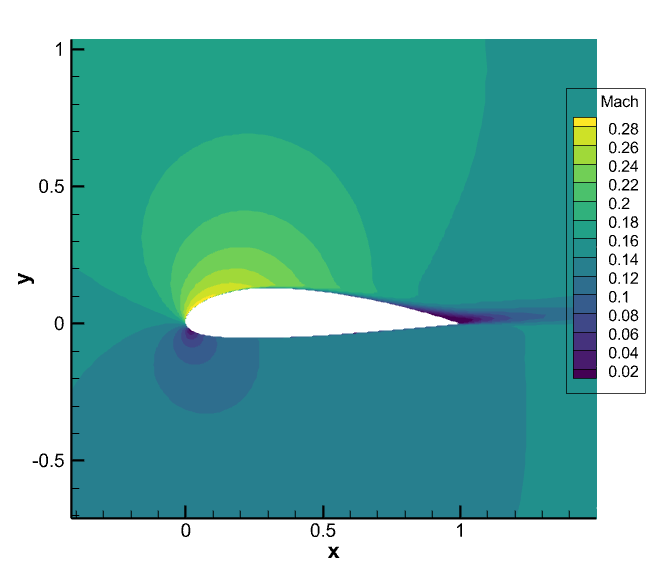
\includegraphics[width=\textwidth, height=0.75\textwidth, 
	scale=1]{takeoff_baseline_Mach} 
	\end{subfigure}
	\hfill
	\begin{subfigure}[b]{0.49\textwidth}
	\centering
	\caption{Pressure field}
	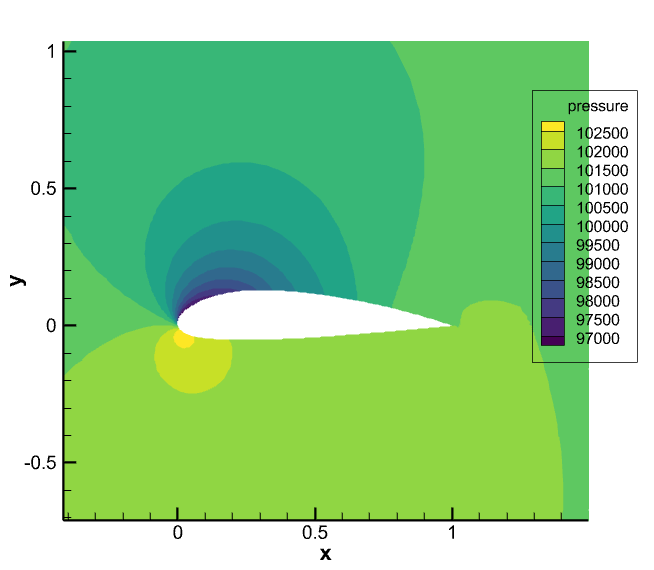
\includegraphics[width=\textwidth, height=0.75\textwidth, 
	scale=1]{takeoff_baseline_pressure}   
	\end{subfigure}
\caption{Flow field quantities of the baseline airfoil geometry}
\label{fig:flow_field_takeoff} 
\end{figure}

The airfoil is subsequently optimized w.r.t. two objectives, 
minimization of the produced drag force and maximization of the 
produced lift force, while no constraint is imposed. The 
optimization problem solved is the following:
\begin{equation}
\begin{split}
& max \hspace{2mm} f_{1}(\vec{β}) = L
\\ &
min \hspace{2mm} f_{2}(\vec{β}) = D
\end{split}
\end{equation}
\\
where the bounds of the design variables shaping the pressure side 
of the airfoil are $-0.26 \leq β_{1-5} \leq -0.24$, while the 
design variables shaping the camber line and the suction side are 
$-0.01 \leq β_{6-8} \leq 10.0$ and $0.24 \leq β_{9-13} \leq 0.26$, 
respectively. 

\newpage
%----------------------------------------------------------------


The optimization is performed via the use EAs and MAEAs, where 
$λ \!= \!40$ offspring are evaluated in each generation and $μ \!= 
\!20$ parents are retained, 3 of which are combined to create a new 
offspring at the start of every new generation. In the optimization 
of the airfoil using MAEAs with on-line training, the LCPE phase 
is initialized after 60 CFD evaluations and uses KPLS and RBFs 
metamodels that are trained via SMT and EASY, respectively. 
Both methods terminate after 400 CFD evaluations have been 
performed and are subsequently compared with to MAEAs using KPLS 
trained off-line on $n_{doe} \!= \!80$ initial training patterns. 
The evolution in all methods retains 15 prominent solutions that 
are stored in the temporary elite set $P_{e}$, which at the end of 
the evolution stores the Pareto frontier of non-dominated 
solutions. Three Pareto fronts are produced via the use of a RNG 
seed number that corresponds to a different offspring population 
$P_{λ}^0$ and are presented in figure \ref{fig:Pareto_takeoff}; 
the set $P_{λ}^{0}$ contains the baseline airfoil geometry.

\begin{figure}[h!]
\centering
\begin{subfigure}[b]{0.49\textwidth}
\centering
\caption{RNG1}
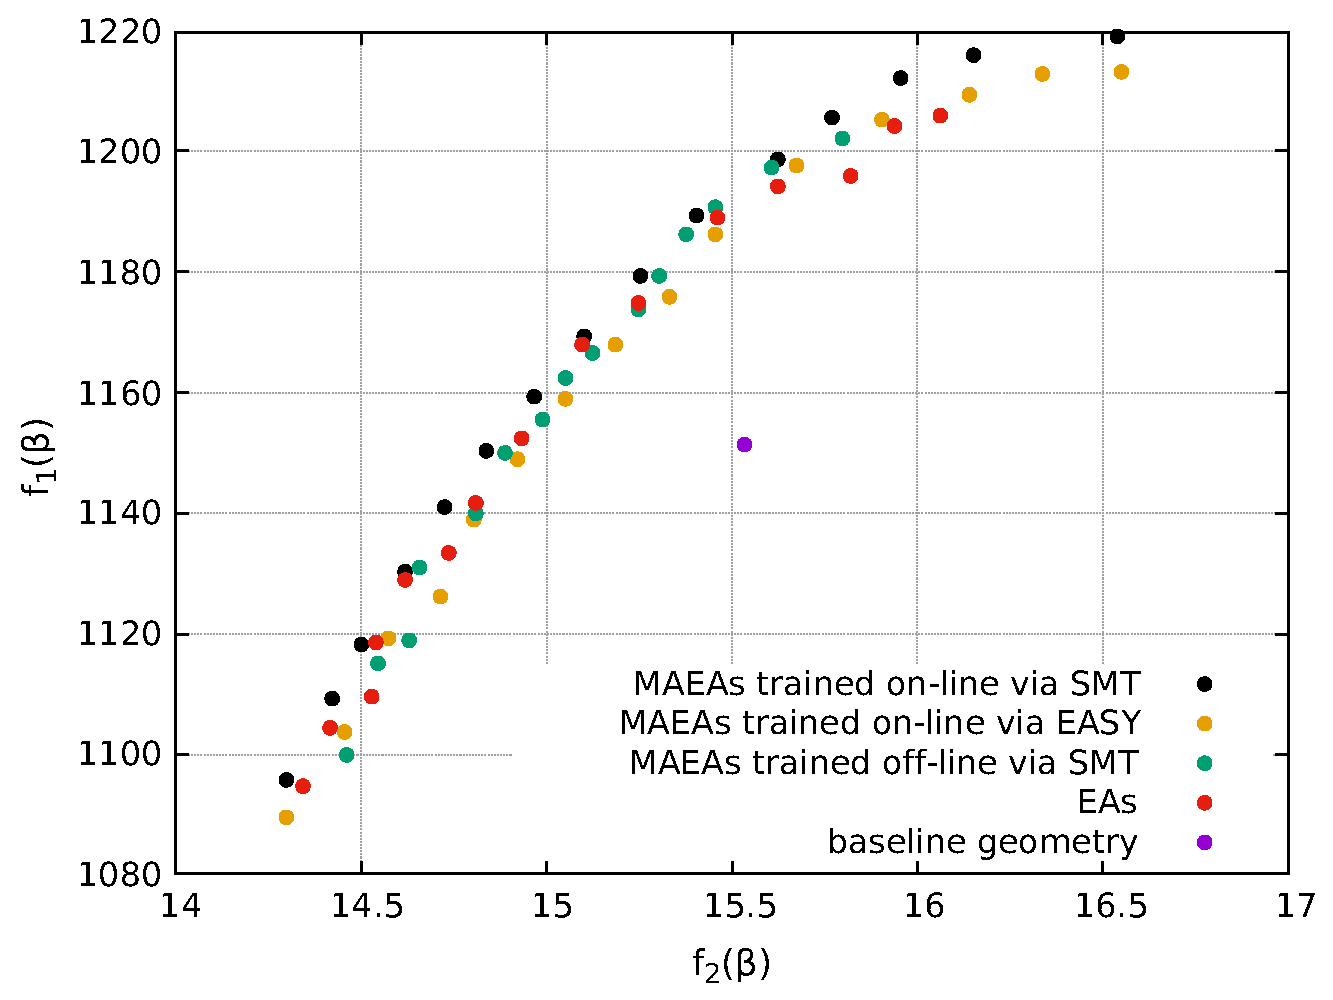
\includegraphics[width=\textwidth, height=0.8\textwidth]
{airfoil_takeoff_MOO_RNG1.pdf}
\end{subfigure}
\hfill
\begin{subfigure}[b]{0.49\textwidth}
\centering
\caption{RNG2}
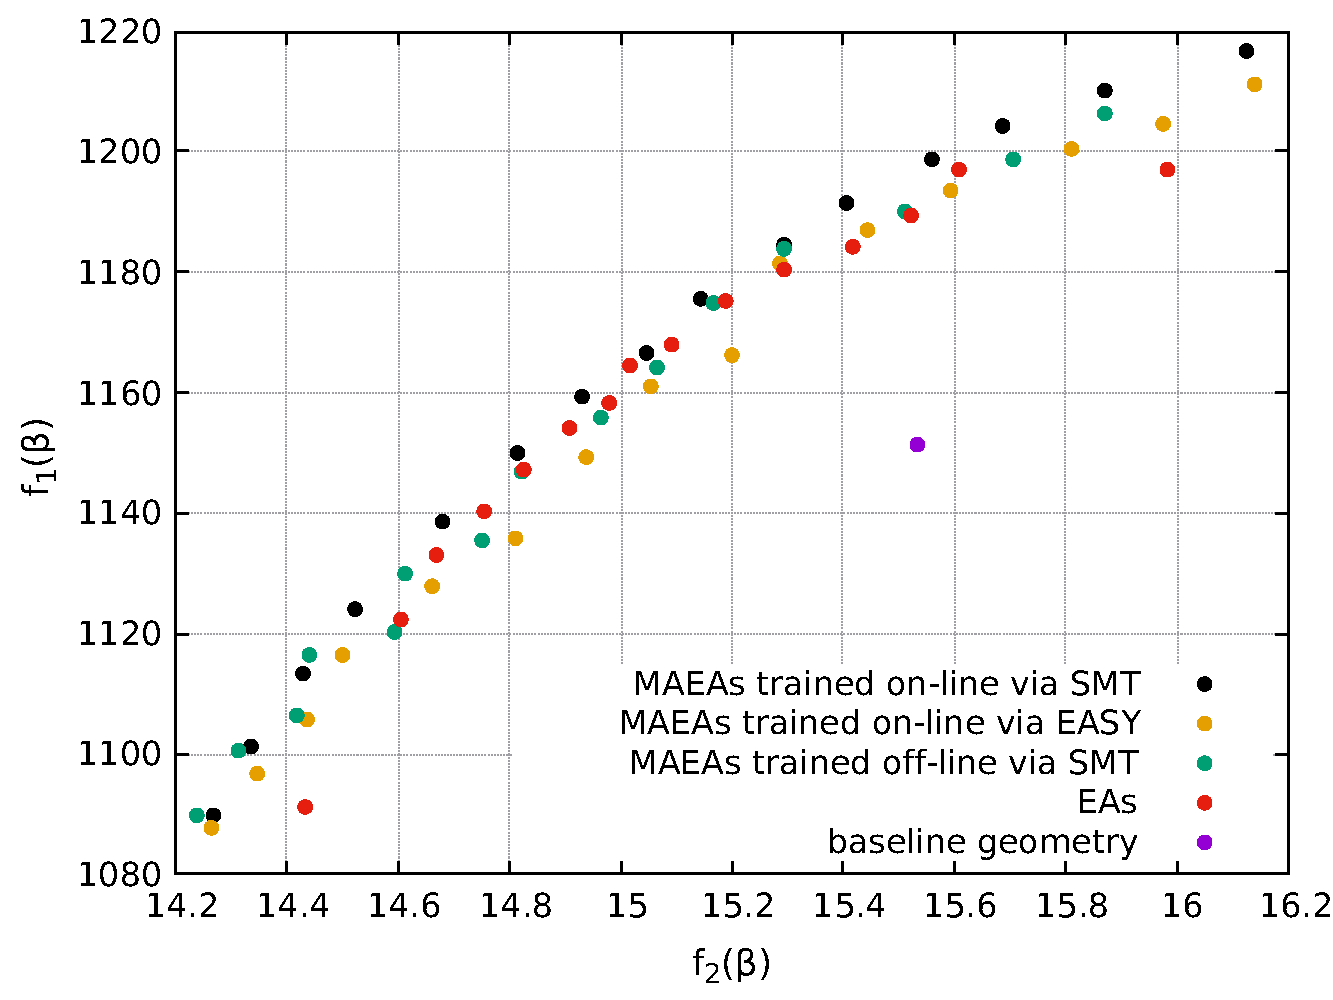
\includegraphics[width=\textwidth, height=0.8\textwidth]
{airfoil_takeoff_MOO_RNG2.pdf}
\end{subfigure}
\hfill
\begin{subfigure}[b]{0.49\textwidth}
\centering
\caption{RNG3}
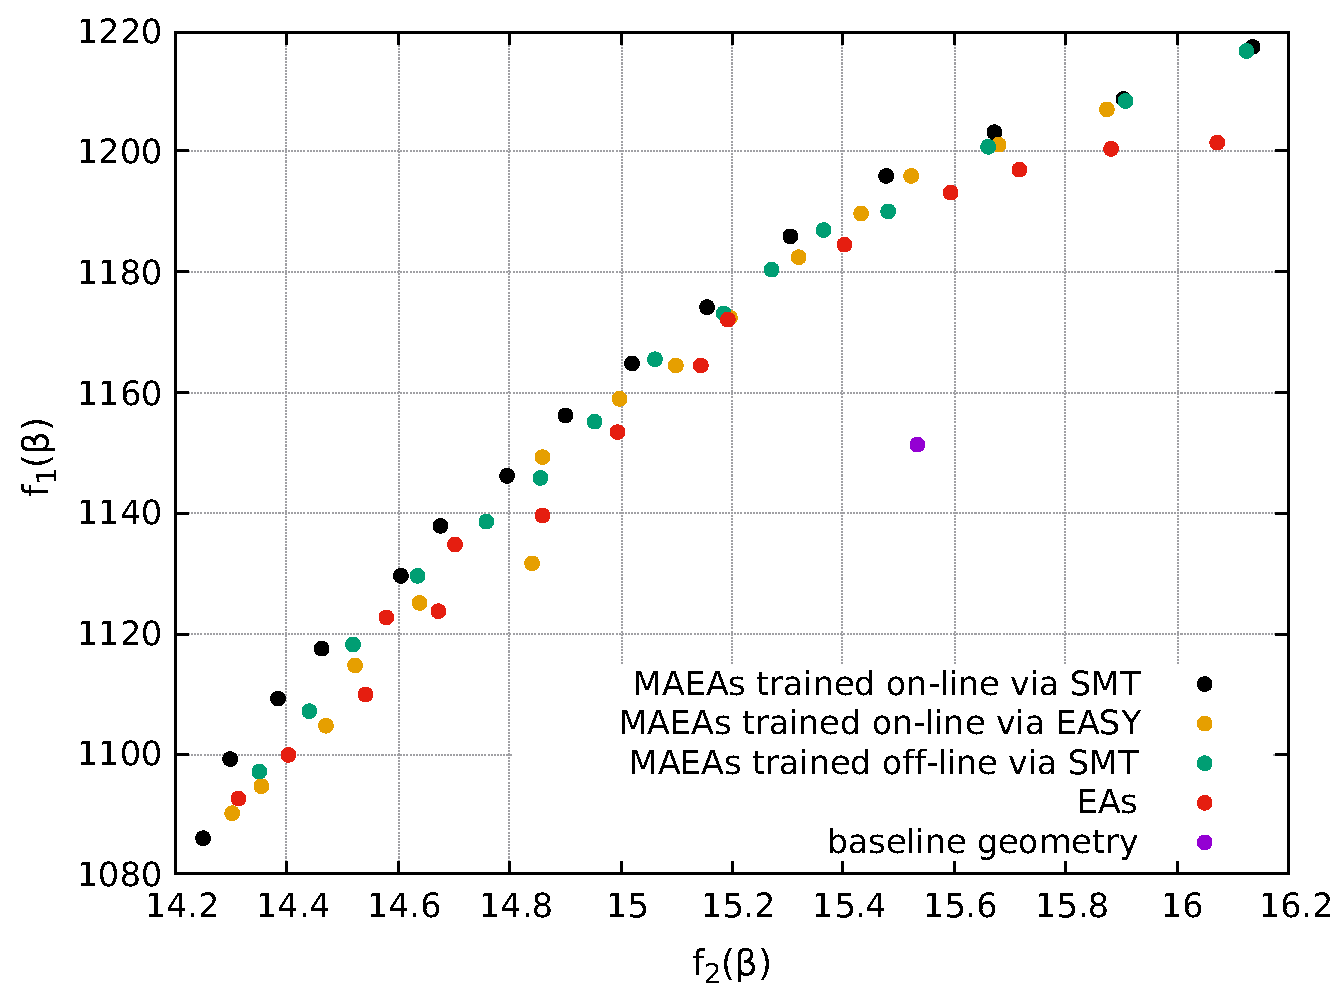
\includegraphics[width=\textwidth, height=0.8\textwidth]
{airfoil_takeoff_MOO_RNG3.pdf}
\end{subfigure}   
\caption{NACA 4318 optimization at take-off flow conditions. 
Comparison of the Pareto fronts of 15 non-dominated solutions 
computed via the implementation of plain EAs, MAEAs with off-line 
and on-line trained KPLS and MAEAs with EASY built-in, on-line 
trained RBFs for 400 CFD evaluations} 
\label{fig:Pareto_takeoff}
\end{figure}


\newpage
%----------------------------------------------------------------


The optimization initialized with seed number RNG1 is allowed to 
perform more CFD evaluations and for this reason the corresponding 
Pareto front contains slightly better non-dominated individuals. In
each case, the Pareto fronts formed via the implementation of each
optimization method do not reveal which method is dominant and 
therefore a hypervolume indicator is assigned to each front 
$\mathcal{F} \subset \mathbb{R}^{n}$.

In the 2D space, which is the case here, the hypervolume indicator
$H(\mathcal{F})$ is equivalent to the area defined by each $\vec{q} 
\in \mathcal{F}$ and the reference point $\vec{x}_{r} \!\in \!
\mathbb{R}^{n}$ is defined as such:
\begin{equation}
\begin{split}
& x_{r_{1}} \!= \! \{ q_{1} \in \mathcal{F}_{i}: q_{1} \geq ξ, 
\forall ξ \in \mathcal{F}_{i}, \forall i \in [1, n_{f}] \} + ξ_{1}
\\ &
x_{r_{2}}  \!= \! \{ q_{2} \in \mathcal{F}_{i}: q_{2} \geq ξ, 
\forall ξ \in \mathcal{F}_{i}, \forall i \in [1, n_{f}] \} + ξ_{2}
\end{split}
\end{equation}
\\[-2mm]
In this case, the parameters assume the values $(ξ_{1}, ξ_{2}) = 
(0.25, 20)$ and the outcome is presented in the table 
\ref{table:hypervolume_takeoff}.

\begin{table}[h!]
\centering
%\rowcolors{2}{gray!30!}{white!50!gray!10}
\scalebox{0.85}{%
\begin{tabular}[c]{ |p{7.3cm}||p{2cm}|p{2cm}|p{2cm}|}
\toprule
\multicolumn{4}{|c|}{\cellcolor{gray!30!} 
\textbf{Hypervolume indicator} $\mathbf{H(\bm{\mathcal{F})}}$} \\
\midrule 
& \textbf{RNG1} & \textbf{RNG2} & \textbf{RNG3} 
\\
\hline
\textbf{MAEAs, on-line training via SMT} & 274.588 & 222.513 
& 224.786 \\
\textbf{MAEAs, on-line training via EASY} & 257.987 & 206.800 
& 211.937 \\
\textbf{MAEAs, off-line training via SMT} & 252.866 & 213.701 
& 216.461 \\
\textbf{EAs} & 257.512 & 200.114 & 204.289 \\
\bottomrule
\end{tabular}%
}
\caption{NACA 4318 optimization at take-off flow conditions. 
Hypervolume indicator of Pareto fronts formed via the 
implementation of various optimization methods}
\label{table:hypervolume_takeoff}
\end{table} 

%\vspace{-4mm}
%\begin{figure}[h!]
%\centering%
%	\begin{subfigure}[b]{0.49\textwidth}%
%	\centering
%	\caption{MAEAs, on-line training via SMT}
%	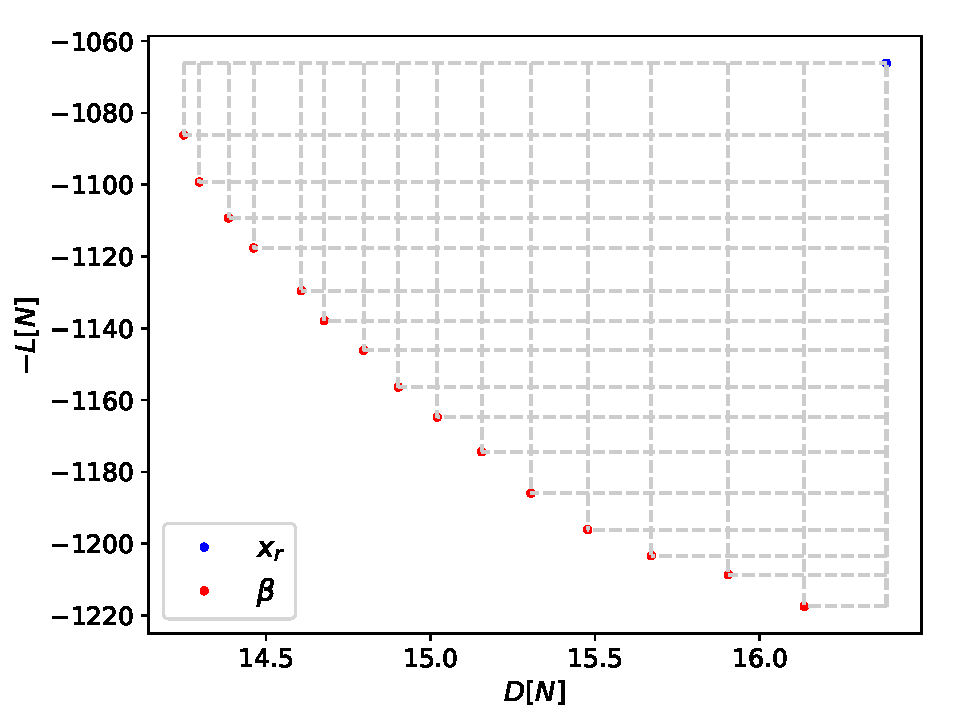
\includegraphics[width=\textwidth, height=0.7\textwidth, 
%	scale=1]{takeoff_MOO_Pareto_front_SMT.pdf} 
%	\end{subfigure}
%	\hfill
%	\begin{subfigure}[b]{0.49\textwidth}
%	\centering
%	\caption{MAEAs, on-line training via EASY}
%	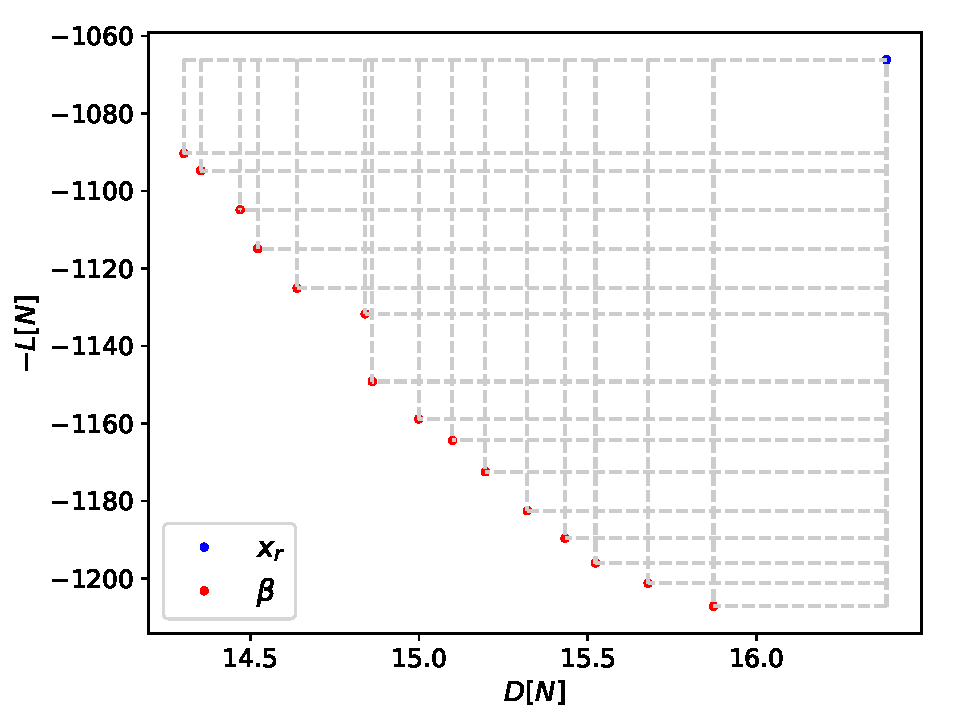
\includegraphics[width=\textwidth, height=0.7\textwidth, 
%	scale=1]{takeoff_MOO_Pareto_front_EASY.pdf}   
%	\end{subfigure}
%	\hfill
%	\begin{subfigure}[b]{0.49\textwidth}
%	\centering
%	\caption{MAEAs, off-line training via SMT}
%	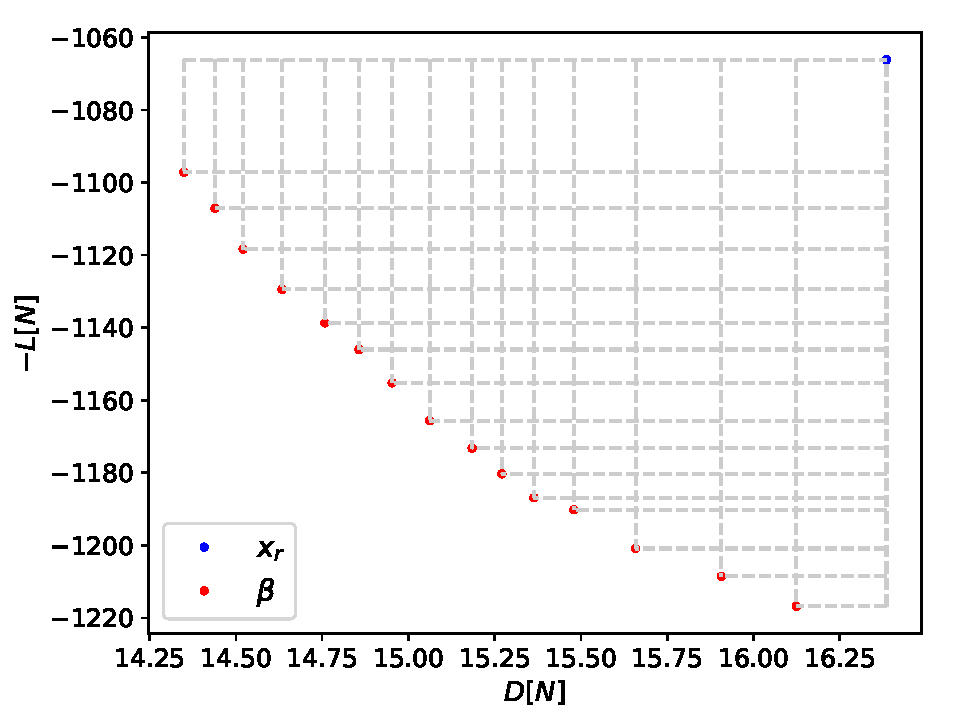
\includegraphics[width=\textwidth, height=0.7\textwidth, 
%	scale=1]{takeoff_MOO_Pareto_front_offline.pdf} 
%	\end{subfigure}
%	\hfill
%	\begin{subfigure}[b]{0.49\textwidth}
%	\centering
%	\caption{EAs}
%	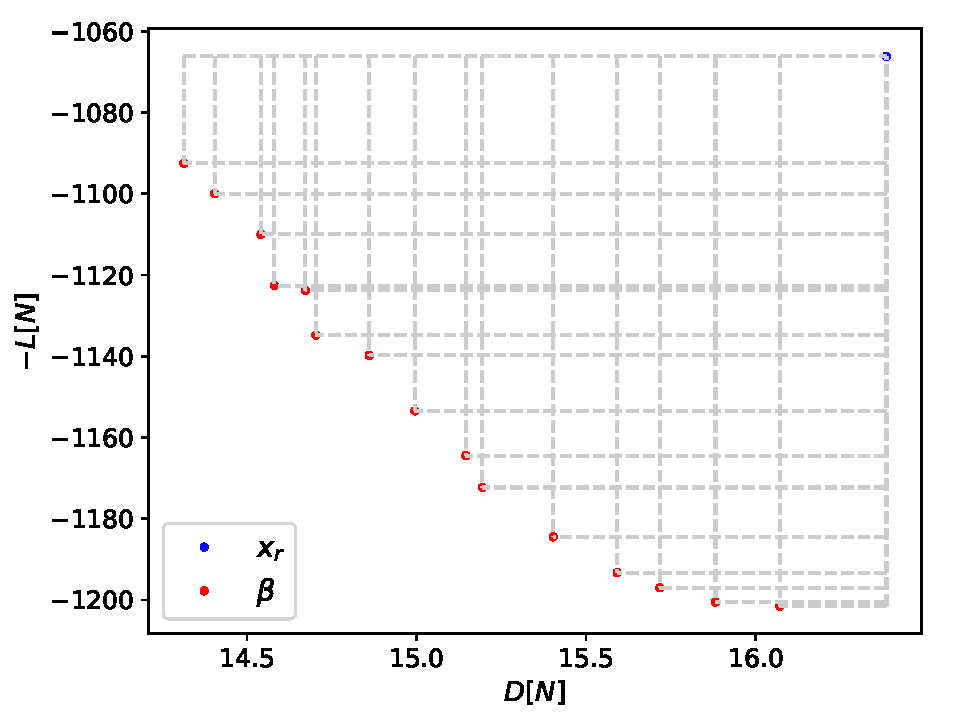
\includegraphics[width=\textwidth, height=0.7\textwidth, 
%	scale=1]{takeoff_MOO_Pareto_front_EAs.pdf}   
%	\end{subfigure}
%\caption{NACA 4318 optimization at take-off flow conditions with 
%RNG3. Comparison between the area defined between each font 
%$\mathcal{F}$ and the reference point $\vec{x}_{r} \!= \!
%(16.39, -1066.14)$} 
%\end{figure}

The Pareto front generated by the implementation of MAEAs with 
metamodels trained on-line via SMT assumes the highest hypervolume 
indicator value for every RNG. On the contrary, the lowest 
hypervolume indicator is observed when the optimization is 
performed via the use plain EAs. MAEAs with off-line training 
perform better than MAEAs with metamodels trained on-line via the 
use of EASY for RNG2, RNG3. For those RNG seed numbers, 
each optimization cycle converges after 1000 evaluations have been 
performed on the trained metamodel, while for RNG1 only 520 
metamodel evaluations are performed. This increase in metamodel 
evaluations has a cost-efficient impact in the efficacy of the 
method and is retained in the following optimization cases.

\newpage
%------------------------------------------------------------------


At take-off conditions the main objective is generating an airfoil
design that produces the maximum lift force; such designs are 
compared in figure \ref{fig:takeoff_MOO_comparison}.

\begin{figure}[h!]
\centering
	\begin{subfigure}[b]{0.49\textwidth}
	\centering
	\caption{MAEAs, on-line training via SMT, 
	\\  $L \!= \!1217.45$ N and $D \!= \!16.14$ N}
	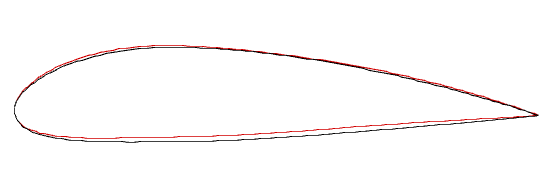
\includegraphics[width=\textwidth, scale=1]{takeoff_MOO_SMT} 
	\end{subfigure}
	\hfill
	\begin{subfigure}[b]{0.49\textwidth}
	\centering
	\caption{MAEAs, on-line training via EASY, 
	\\ $L \!= \!1207.19$ N and $D \!= \!15.87$ N}
	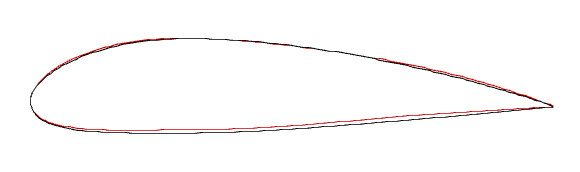
\includegraphics[width=\textwidth, height = 0.35\textwidth, 
	scale=1]{takeoff_MOO_EASY}   
	\end{subfigure}
	\hfill
	\begin{subfigure}[b]{0.49\textwidth}
	\centering
	\caption{MAEAs, off-line training, 
	\\ $L \!= \!1216.79$ N and $D \!= \!16.12$ N}
	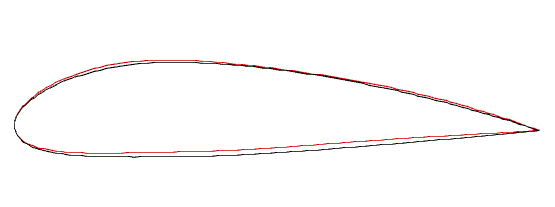
\includegraphics[width=\textwidth, scale=1]{takeoff_MOO_offline} 
	\end{subfigure}
	\hfill
	\begin{subfigure}[b]{0.49\textwidth}
	\centering
	\caption{EAs, $L \!= \!1201.47$ N and $D \!= \!16.07$ N}
	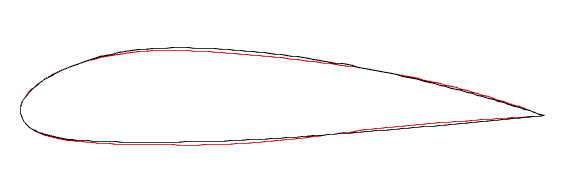
\includegraphics[width=\textwidth, height = 0.38\textwidth, 
	scale=1]{takeoff_MOO_EAs}   
	\end{subfigure}
\caption{NACA 4318 optimization at take-off conditions with RNG3. 
Comparison between airfoil desings that yield the highest lift 
force in the Pareto front (red) compared to the baseline design 
(black).} 
\label{fig:takeoff_MOO_comparison}
\end{figure}

The use of MAEAs with metamodels trained on-line via SMT result 
in both the optimal Pareto front and the best optimal solution. In 
the relative ranking of each method, MAEAs using metamodels trained
off-line via SMT finish second when considering their reduced 
computational cost.


\newpage
%------------------------------------------------------------------


\subsection{SOO optimization at take-off conditions}
The second optimization case focuses on the maximization of the 
produced lift force when the airfoil operates at take-off 
conditions. In this case, however, the maximization of the lift 
force is the only objective of the optimization and the design 
space solutions is bounded by a user-imposed demand of a less than
$8 \%$ increase in drag force produced compared to the initial 
baseline geometry, where $D_{bsl} \!= \!15.53$ N. The constrained 
SOO can be expressed as such: 
\begin{equation}
\begin{split}
max \hspace{2mm} & f(\vec{β}) = L
\\[0.2cm] 
\text{subject to} \hspace{2mm} & c_{1}(\vec{β}) = 
D - 1.08D_{bsl} \leq 0
\end{split}
\end{equation}
\\
with bounds of the design variables identical to the ones used in 
the MOO case.
 
The optimization is performed via the use EAs and MAEAs, where $λ 
\!= \!40$ offspring are evaluated in each generation and $μ \!= \!
20$ parents are retained, 3 of which are combined to create a new 
offspring at the start of every new generation. In the optimization 
of the airfoil using MAEAs with on-line training, the LCPE phase 
is initialized after 40 CFD evaluations. Both optimization methods 
terminate after 400 CFD evaluations have been performed. Based on 
the outcome of the MOO optimization case, the initial offspring 
population $P_{λ}^0$ is produced via the use of a RNG2 and RNG3 
seed; the set $P_{λ}^{0}$ contains the baseline airfoil geometry.
The convergence history of RNG3 optimization using plain EAs and 
MAEAs with on-line training is presented in figure 
\ref{fig:online_takeoff_SOO}.

\begin{figure}[h!]
\centering
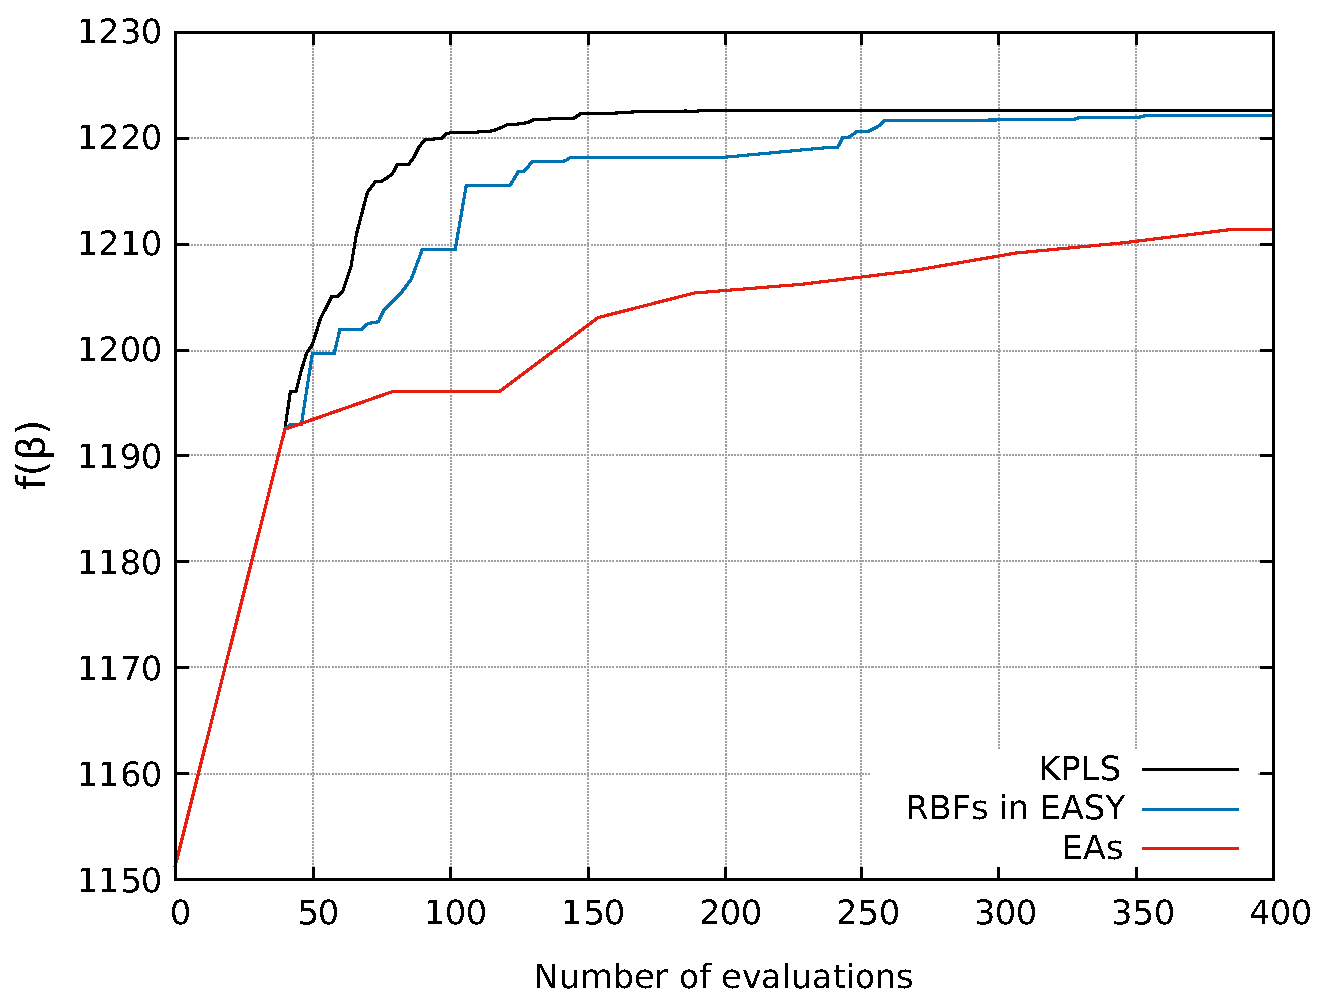
\includegraphics[width=0.6\textwidth]{takeoff_SOO_convergence.pdf}   
\caption{Maximizing NACA 4318 lift force at take-off conditions 
using RNG3. Comparison between the convergence histories of plain 
EAs and MAEAs with metamodels trained on-line via SMT and EASY} 
\label{fig:online_takeoff_SOO}
\end{figure}

Both MAEA methods outperform conventional EAs in the number of CFD 
evaluations performed. The optimization facilitated by MAEAs 
with surrogate models trained on-line via SMT, however, has 
seemingly the best convergence speed, since it converges to the 
optimal solution after performing circa 150 CFD evaluations.

\newpage
%------------------------------------------------------------------


Both methods are subsequently compared with to MAEAs using KPLS 
trained off-line on $n_{doe} \!= \!80$ initial training patterns, 
in order to determine which method is more efficient. The 
optimization processin MAEAs with off-line training converges after 
1000 evaluations per cycle have been perfomed on the surrogate 
model, in this case KPLS. At the end of each cycle $n_{new\_doe} = 
5$ random training patterns are sampled.

\begin{figure}[h!]
\centering
	\begin{subfigure}[b]{0.45\textwidth}
	\centering
	\caption{MAEAs, on-line training via SMT, 
	\\  $L \!= \!1222.52$ N and $D \!= \!16.54$ N}
	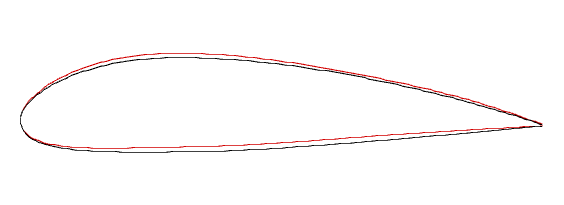
\includegraphics[width=\textwidth]{takeoff_SOO_SMT} 
	\end{subfigure}
	\hfill
	\begin{subfigure}[b]{0.45\textwidth}
	\centering
	\caption{MAEAs, on-line training via EASY, 
	\\ $L \!= \!1222.06$ N and $D \!= \!16.44$ N}
	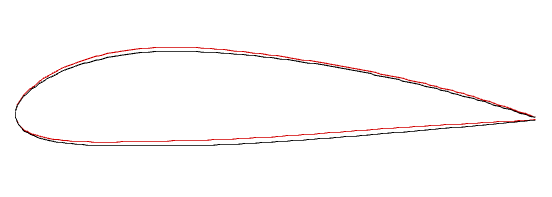
\includegraphics[width=\textwidth, scale=1]{takeoff_SOO_EASY}   
	\end{subfigure}
	\hfill
	\begin{subfigure}[b]{0.45\textwidth}
	\centering
	\caption{MAEAs, off-line training via SMT, 
	\\ $L \!= \!1221.02$ N and $D \!= \!16.29$ N}
	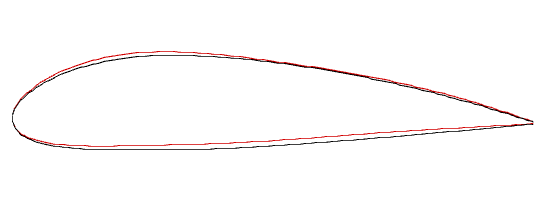
\includegraphics[width=\textwidth, scale=1]{takeoff_SOO_offline} 
	\end{subfigure}
	\hfill
	\begin{subfigure}[b]{0.45\textwidth}
	\centering
	\caption{EAs, $L \!= \!1211.35$ N and $D \!= \!16.25$ N}
	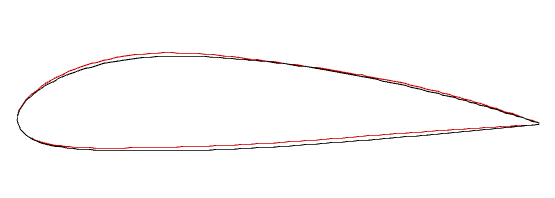
\includegraphics[width=\textwidth, scale=1]{takeoff_SOO_EAs}   
	\end{subfigure}
\caption{NACA 4318 optimization at take-off conditions with RNG3. 
Comparison between optimal airfoil desings.} 
\label{fig:takeoff_SOO_designs}
\end{figure}

All optimized designs in figure \ref{fig:takeoff_SOO_designs} 
result in a positive displacement of the camber line. In the 
suction side, the increase in curvature near the leading edge of 
the airfoil results in an increase of the favourable pressure 
gradient $dp/dx < 0$. The adverse pressure gradient $dp/dx > 0$ in 
the suction side, which is responsible for the turbulence 
generation, remains relatively unchanged to prevent the flow 
separation in the boundary layer. In the pressure side, an increase 
in the pressure gradient is desired and is achieved via an increase 
in the airfoil curvature. The pressure field of the optimized 
airfoil is presented next, where the optimized airfoil shows a 
$6.1 \%$ increase in lift force $L$ and a $4.5 \%$ increase in 
drag force $D$, as shown in figure 
\ref{fig:takeoff_SOO_before_after}.

\begin{figure}[h!]
\centering
	\begin{subfigure}[b]{0.49\textwidth}
	\centering
	\caption{Baseline}
	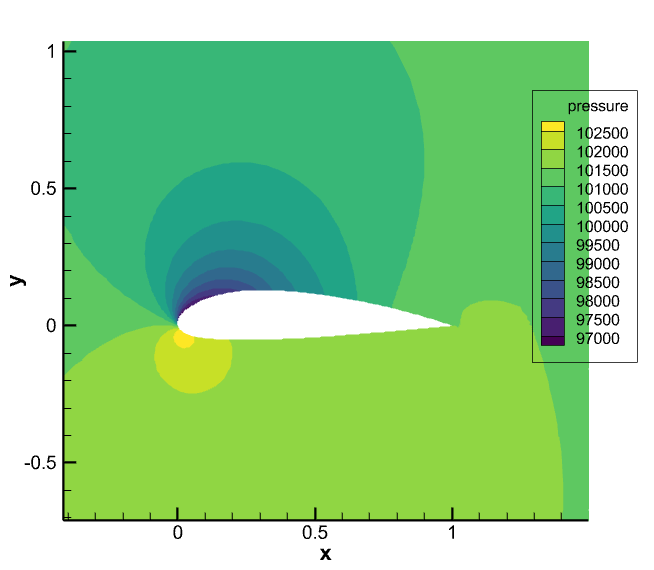
\includegraphics[width=\textwidth, height=0.64\textwidth, 
	scale=1]{takeoff_baseline_pressure} 
	\end{subfigure}
	\hfill
	\begin{subfigure}[b]{0.49\textwidth}
	\centering
	\caption{Optimized via MAEAs with metamodels trained off-line}
	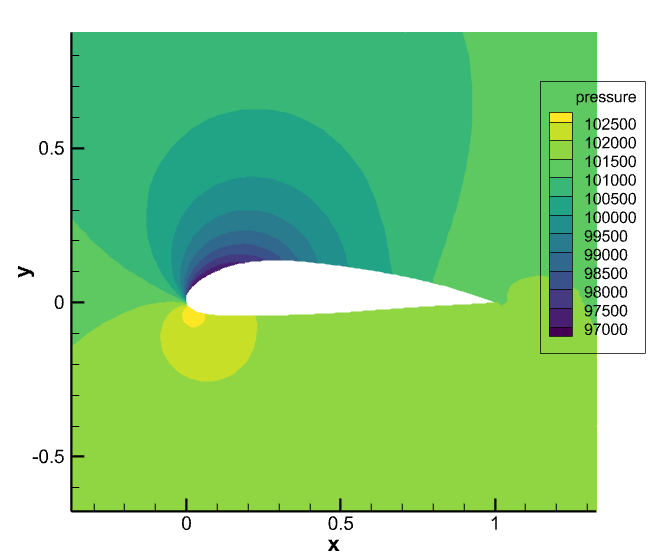
\includegraphics[width=\textwidth, height=0.64\textwidth, 
	scale=1]{takeoff_SOO_offline_pressure}   
	\end{subfigure}
\caption{Comparison between baseline and optimized airfoil} 
\label{fig:takeoff_SOO_before_after}
\end{figure}

\newpage
%----------------------------------------------------------------


In the current airfoil shape optimization cases, the PSM is the CFD 
solver. A single CFD evaluation, which is combined with some 
subprocess related to the adaptation of the mesh around the new 
airfoil design, is far more costly than any PSM evaluation 
performed in previous pseudo-engineering optimization cases and  
metamodel predictions. For this reason, $\overline{n}_{PSM}$ alone 
significantly increases the computational cost. For the sake of 
completeness, however, the total functions calls, i.e. 
$\overline{n}_{PSM}$ and $\overline{n}_{meta}$, and the average 
outcome produced via the implementation of each method are 
presented in table \ref{table:takeoff_outcome}, in order to ensure 
that the best possible optimization method is selected.

\begin{table}[h!]
\centering
%\rowcolors{2}{gray!30!}{white!50!gray!10}
\scalebox{0.83}{%
\begin{tabular}[c]{ |p{7.3cm}||p{2.6cm}|p{1.3cm}|p{1.3cm}|}
\toprule
\multicolumn{4}{|c|}{\cellcolor{gray!30!}
\textbf{NACA 4318 optimization at take-off conditions}} \\
\midrule 
& \textbf{Average} $\vec{\mathbf{f}}$ 
& $\mathbf{\overline{n}_{PSM}}$ & $\mathbf{\overline{n}_{meta}}$ \\
\hline
\textbf{MAEAs, on-line training via SMT} & 1222.33 & 400
& 2988 \\
\textbf{MAEAs, on-line training via EASY} & 1221.90 & 400 
& 4000 \\
\textbf{MAEAs, off-line training via SMT} & 1221.27 & 81 
& 1000 \\
\textbf{EAs} & 1211.54 & 400 & - \\
\bottomrule
\end{tabular}%
}
\caption{Comparison between all implemented optimization methods}
\label{table:takeoff_outcome}
\end{table}


%\begin{table}[h!]
%\centering
%%\rowcolors{2}{gray!30!}{white!50!gray!10}
%\scalebox{0.81}{%
%\begin{tabular}[c]{ |p{2.4cm}||p{1.8cm}|p{1.2cm}|p{1.2cm}|
%p{1.8cm}|}
%\toprule
%\multicolumn{5}{|c||}{\cellcolor{gray!30!} 
%\textbf{NACA 4318 optimization at take-off conditions}} \\
%\midrule 
%& \textbf{Wall clock time/process [s]} 
%& $\mathbf{\overline{n}_{PSM}}$ & $\mathbf{\overline{n}_{meta}}$
%& \textbf{Total wall clock time [s]} \\
%\hline
%\multicolumn{5}{|c|}{\cellcolor{gray!15!} \textbf{EAs}} \\
%\textbf{CFD eval.} & 450 & 400 & - & 180000 \\
%\hline
%\multicolumn{5}{|c|}{\cellcolor{gray!15!} \textbf{MAEAs, off-line 
%training via SMT}} \\
%\textbf{Sampling} & 0.859 & - & 1 & 0.859 \\
%\textbf{CFD eval.} & 450 & 81 & - & 36450 \\
%\textbf{F Training} & 1.423 & - & 1 & 1.423 \\
%\textbf{C training} & 1.563 & - & 1 & 1.563 \\
%\textbf{Prediction} & 1.547 & - & 1000 & 1547 \\
%\hline
%\multicolumn{5}{|c|}{\cellcolor{gray!15!} \textbf{MAEAs, on-line 
%training via SMT}} \\
%\textbf{PSM eval.} & 450 & 400 & - & 180000 \\
%\textbf{Training} & 1.443 & - & 2988 & 4311.684 \\
%\textbf{Prediction} & 1.137 & - & 2988 & 3397.356 \\
%\hline
%\multicolumn{5}{|c|}{\cellcolor{gray!15!} \textbf{MAEAs, on-line 
%training via EASY}} \\
%\textbf{PSM eval.} & 450 & 400 & - & 180000 \\
%\textbf{Training} & 0.257 & - & 4000 & 1028 \\
%\textbf{Prediction} & 0.102 & - & 4000 & 408 \\
%\bottomrule
%\end{tabular}%
%}
%\caption{Wall clock time of each individual process as measured 
%when using the KPLS model}
%\end{table}

The total wall clock time of the optimization is significantly 
decreased when MAEAs with off-line training are implemented and 
their corresponding outcome is similar to the one obtained via the 
implementation of MAEAs with on-line training. Consequently, the 
lift force $L$ of the NACA 4318 at take-off conditions is maximized 
when MAEAs with off-line training are implemented, followed closely 
by MAEAs with surrogate models trained on-line via SMT that yield 
an optimal solution after circa 150 CFD evaluations have been 
performed. 


\newpage
%---------------------------------------------------------------


\subsection{SOO optimization at cruise conditions}
The last optimization case simulates the conditions governing the 
cruise stage of an aircraft flight, which are characterized by 
high free-stream velocity $U \!= \!206.64$ $m/s$, low angle of 
attack $a \!= \!2^o$ and fluid properties at sea level given in 
table \ref{table:cruise_height}. 

\begin{table}[h!]
\centering
%\rowcolors{2}{gray!30!}{white!50!gray!10}
\scalebox{0.83}{%
\begin{tabular}[c]{ |p{1.5cm}||p{2.2cm}|p{2.2cm}|p{2.2cm}|}
\toprule
\multicolumn{4}{|c|}{\cellcolor{gray!30!} 
\textbf{Fluid properties at h = 11000 m}} \\
\midrule 
& $\bm{ρ}$ $\mathbf{[kg/m^3]}$ & \textbf{p [bar]} & \textbf{T [K]} 
\\
\hline
\textbf{Air} & 0.364805 & 0.227 & 216.8 \\
\bottomrule
\end{tabular}%
}
\caption{Air properties at cruise height}
\label{table:cruise_height}
\end{table} 

\vspace{-2mm}

In this case, the minimization of the produced drag force is the 
only objective of the optimization and the design space 
is bounded by a user-imposed demand of a less than $8 \%$ 
decrease in lift force compared to the initial baseline geometry, 
where $L_{bsl} \!= \!1123.81$ N. The constrained SOO can be 
expressed as such: 
\begin{equation}
\begin{split}
min \hspace{2mm} & f(\vec{β}) = D
\\[0.1cm] 
\text{subject to} \hspace{2mm} & c_{1}(\vec{β}) = 
L - 0.92L_{bsl} \geq 0
\end{split}
\end{equation}
\\
with bounds of the design variables identical to the ones used in 
the MOO case.  

The optimization is performed via the use EAs and MAEAs, where $λ 
\!= \!40$ offspring are evaluated in each generation and $μ \!= \!
20$ parents are retained, 3 of which are combined to create a new 
offspring at the start of every new generation. In the MAEA-based 
optimization of the airfoil using on-line training, the LCPE phase 
is initialized after 40 CFD evaluations. Both optimization methods 
terminate after 400 CFD evaluations have been performed. The 
initial population set $P_{λ}^0$ is produced via the use of a 
RNG2 and RNG3 seed; the set $P_{λ}^{0}$ contains the baseline 
airfoil geometry. The convergence history of RNG3 optimization 
using plain EAs and MAEAs with on-line training is presented in 
figure \ref{fig:online_cruise}.

\begin{figure}[h!]
\centering
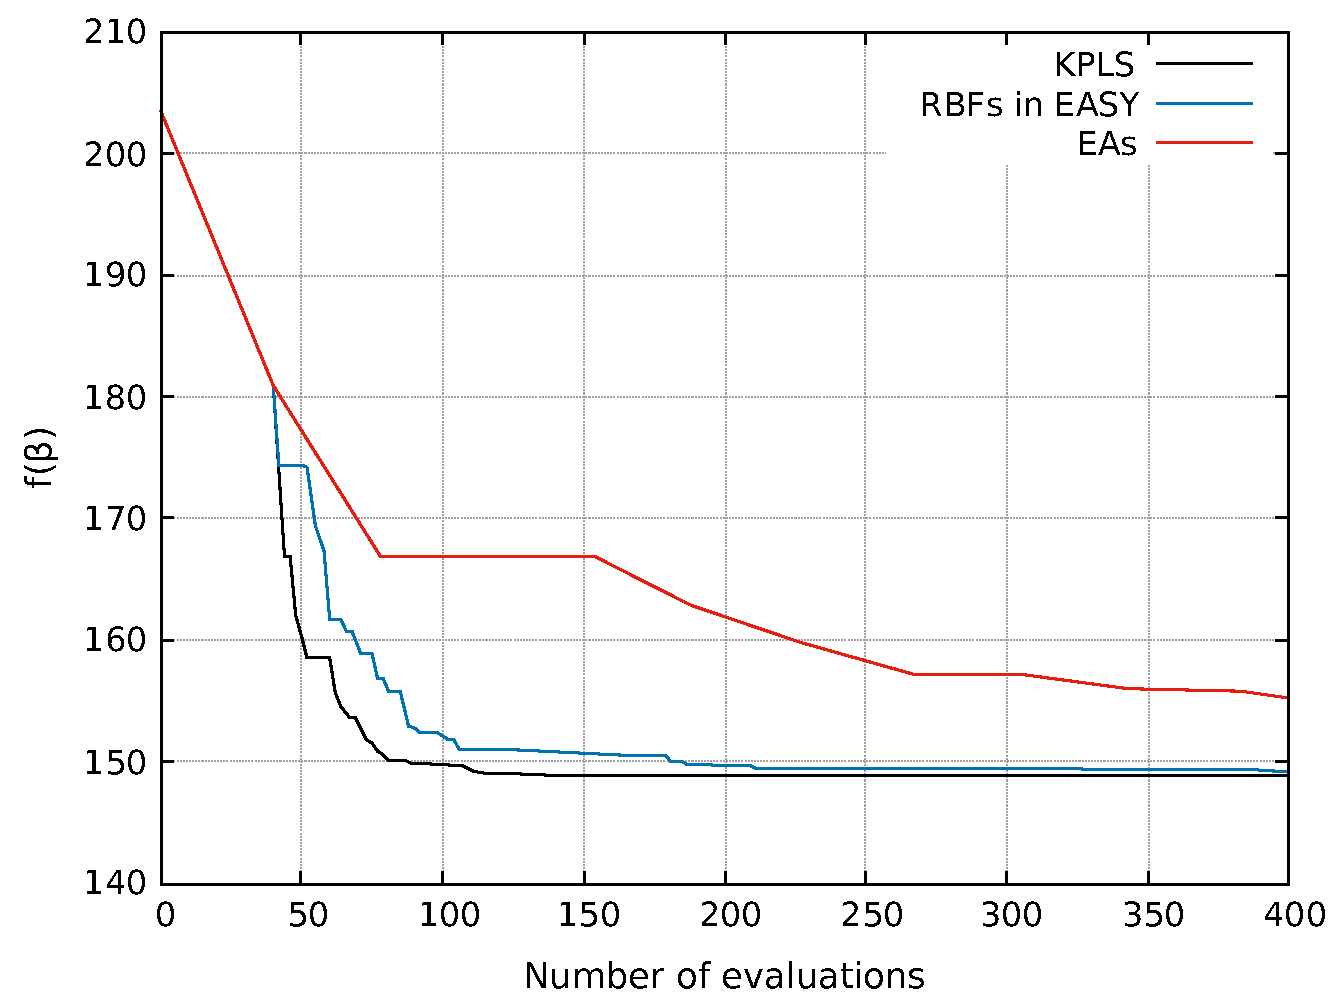
\includegraphics[width=0.55\textwidth]{cruise_SOO_convergence.pdf}   
\caption{Minimizing NACA 4318 drag force at cruise conditions 
with RNG3. Comparison between the convergence histories of plain 
EAs and MAEAs with metamodels trained on-line via SMT and EASY}
\label{fig:online_cruise} 
\end{figure}

\newpage
%----------------------------------------------------------------


Both MAEA methods outperform conventional EAs in the number of CFD 
evaluations performed. The optimization facilitated by MAEAs with 
surrogate models trained on-line via SMT, however, has seemingly 
the best convergence speed, since it converges to the optimal 
solution after performing circa 150 CFD evaluations.
 
Both methods subsequently compared with to MAEAs using KPLS 
trained off-line on $n_{doe} \!= \!80$ initial training patterns, 
in order to determine which method is more efficient. The 
optimization process in MAEAs with off-line training converges 
after 1000 evaluations have been perfomed per cycle on the 
surrogate model, in this case KPLS. At the end of each cycle 
$n_{new\_doe} = 5$ random training patterns are sampled.

\begin{figure}[h!]
\centering
	\begin{subfigure}[b]{0.49\textwidth}
	\centering
	\caption{MAEAs, on-line training via SMT, 
	\\  $D \!= \!148.87$ N and $D \!= \!1373.12$ N}
	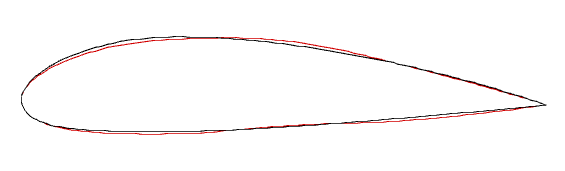
\includegraphics[width=\textwidth, scale=1]{cruise_SMT} 
	\end{subfigure}
	\hfill
	\begin{subfigure}[b]{0.49\textwidth}
	\centering
	\caption{MAEAs, on-line training via EASY, 
	\\ $D \!= \!149.24$ N and $D \!= \!1383.62$ N}
	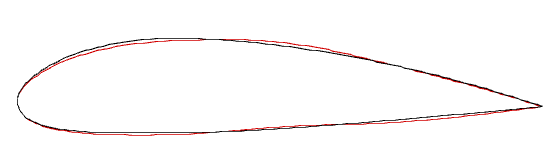
\includegraphics[width=\textwidth, scale=1]{cruise_EASY}   
	\end{subfigure}
	\hfill
	\begin{subfigure}[b]{0.49\textwidth}
	\centering
	\caption{MAEAs, off-line training via SMT, 
	\\ $D \!= \!150.06$ N and $L \!= \!1367.56$ N}
	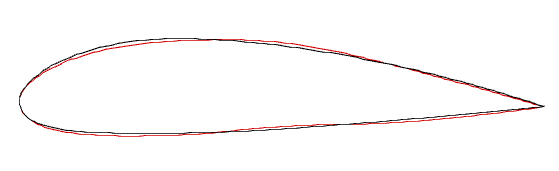
\includegraphics[width=\textwidth, scale=1]{cruise_offline} 
	\end{subfigure}
	\hfill
	\begin{subfigure}[b]{0.49\textwidth}
	\centering
	\caption{EAs, $D \!= \!155.25$ N and $L \!= \!1429.83 N$}
	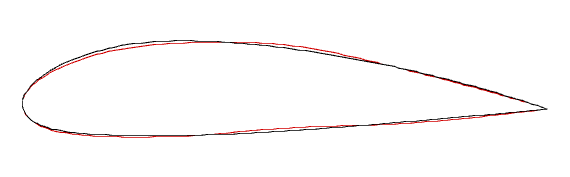
\includegraphics[width=\textwidth, scale=1]{cruise_EAs}   
	\end{subfigure}
\caption{NACA 4318 take-off conditions with RNG3. Comparison 
between airfoil desings that resulted after the implementation of 
each optimization methods.} 
\label{fig:cruise_designs}
\end{figure}

The streamline flow of $Mach \!= \!0.7 $ is accelerated in the 
suction side and becomes supersonic, reaching its peak $Mach 
\!= \!1.3$ for the baseline airfoil as seen in figure 
\ref{fig:cruise_before_after}. As a result, a shock wave is
formed that interacts with the boundary layer and leads to flow 
separation. The aim of the optimization is to delay the formation 
of the shock wave and by extension the flow separation. As depicted 
in figure \ref{fig:cruise_designs}, this can be achieved by 
decreasing the curvature near the leading edge of the 
airfoil, and therefore the favourable pressure gradient 
$dp/dx < 0$. On the other hand, the adverse pressure gradient 
$dp/dx > 0$ is increased by an increase of curvature. The 
pressure side of the optimized airfoil forms a slightly concave 
surface that is formed due to the negative displacement of the 
camber line and results in high pressure region. Flow separation is 
mostly responsible for the induced drag force and thus the 
optimized airfoil designs reduce the flow separation region while
simultaneously increasing the pressure coefficient around the 
airfoil and by extension the produced lift force $L$. In the 
baseline geometry, the flow separation initiates at $x/c \!= \!
0.33$, while in the optimized designs the flow separation initiates 
at $x/c \!= \!0.43$ of the normalized characteristic length. 
As a result the optimized designs show a $26.3 \%$ decrease in drag 
force $D$, combined with a $21.8 \%$ increase in lift force $L$.

\newpage
%-------------------------------------------------------------


\begin{figure}[h!]
\centering
	\begin{subfigure}[b]{0.49\textwidth}
	\centering
	\caption{Baseline Mach field}
	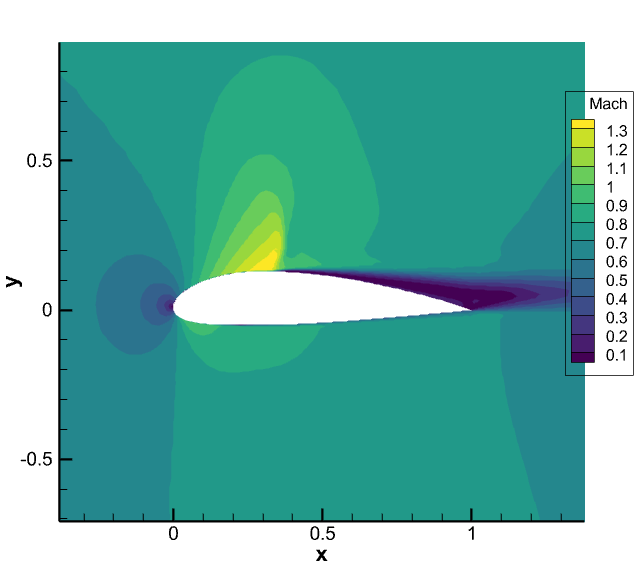
\includegraphics[width=\textwidth, height=0.75\textwidth, 
	scale=1]{cruise_baseline_Mach} 
	\end{subfigure}
	\hfill
	\begin{subfigure}[b]{0.49\textwidth}
	\centering
	\caption{Optimized Mach field via MAEAs with metamodels trained 
	off-line}
	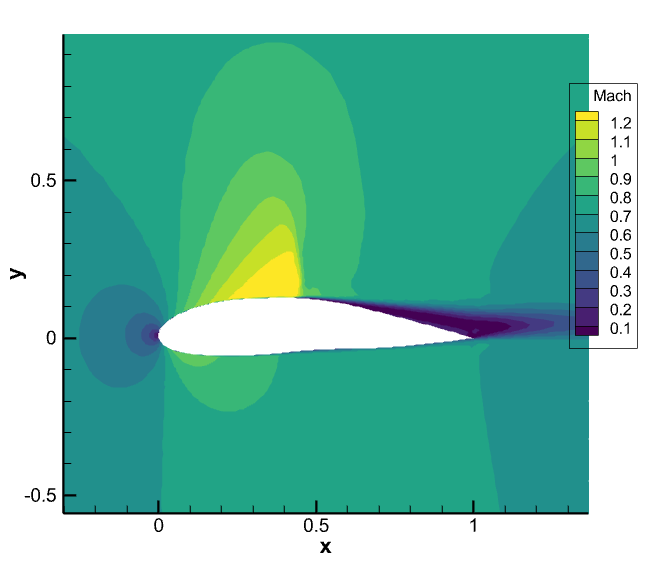
\includegraphics[width=\textwidth, height=0.75\textwidth, 
	scale=1]{cruise_offline_Mach}   
	\end{subfigure}
%	\hfill
%	\begin{subfigure}[b]{0.49\textwidth}
%	\centering
%	\caption{Baseline pressure field}
%	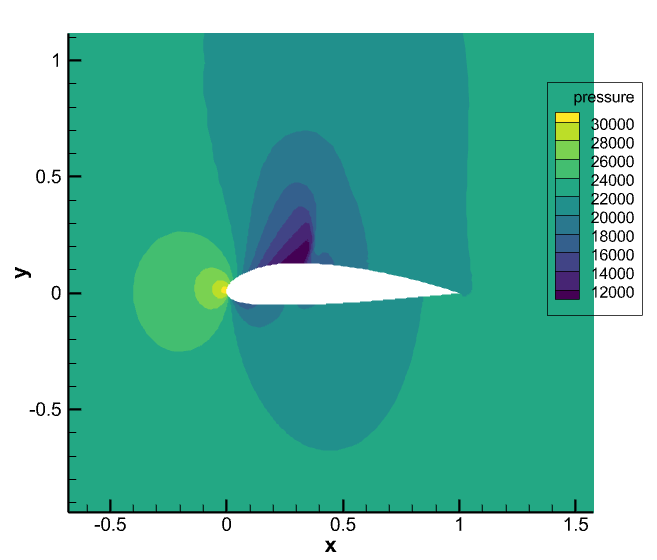
\includegraphics[width=\textwidth, height=0.8\textwidth, 
%	scale=1]{cruise_baseline_pressure}   
%	\end{subfigure}
%	\hfill
%	\begin{subfigure}[b]{0.49\textwidth}
%	\centering
%	\caption{Optimized pressure field via MAEAs with metamodels 
%	trained off-line}
%	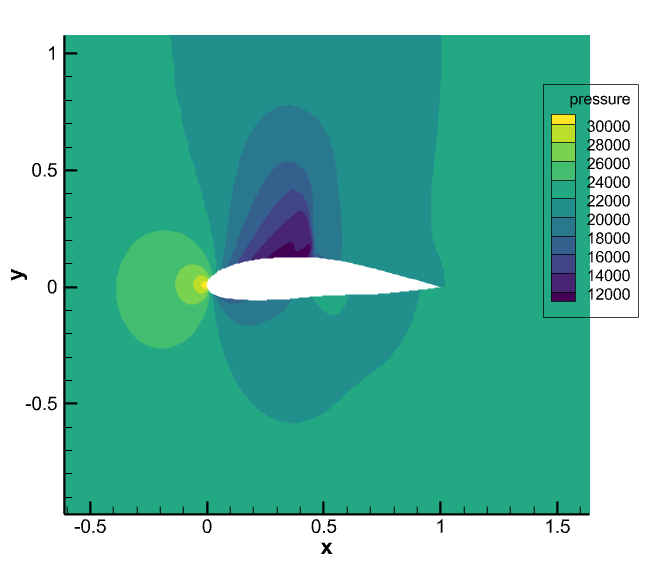
\includegraphics[width=\textwidth, height=0.8\textwidth, 
%	scale=1]{cruise_offline_pressure}   
%	\end{subfigure}
\caption{Comparison between baseline and optimized airfoil} 
\label{fig:cruise_before_after}
\end{figure}


In the current airfoil shape optimization cases, the PSM is the CFD 
solver. A single CFD evaluation, which is combined with some 
subprocess related to the adaptation of the mesh around the new 
airfoil design, is far more costly than any PSM evaluation 
performed in previous pseudo-engineering optimization cases and  
metamodel predictions. For this reason, $\overline{n}_{PSM}$ alone 
significantly increases the computational cost. For the sake of 
completeness, however, the total functions calls, i.e. 
$\overline{n}_{PSM}$ and $\overline{n}_{meta}$, and the average 
outcome produced via the implementation of each method are 
presented in table \ref{table:cruise_outcome}, in order to ensure 
that the best possible optimization method is selected.

\begin{table}[h!]
\centering
%\rowcolors{2}{gray!30!}{white!50!gray!10}
\scalebox{0.83}{%
\begin{tabular}[c]{ |p{7.3cm}||p{2.6cm}|p{1.3cm}|p{1.3cm}|}
\toprule
\multicolumn{4}{|c|}{\cellcolor{gray!30!}
\textbf{NACA 4318 optimization at cruise conditions}} \\
\midrule 
& \textbf{Average} $\vec{\mathbf{f}}$ 
& $\mathbf{\overline{n}_{PSM}}$ & $\mathbf{\overline{n}_{meta}}$ \\
\hline
\textbf{MAEAs, on-line training via SMT} & 148.86 & 400 & 2988 \\
\textbf{MAEAs, on-line training via EASY} & 149.57 & 400 & 4000 \\
\textbf{MAEAs, off-line training via SMT} & 149.60 & 87 & 2000 \\
\textbf{EAs} & 154.63 & 400 & - \\
\bottomrule
\end{tabular}%
}
\caption{Comparison between all implemented optimization methods}
\label{table:cruise_outcome}
\end{table}

%\begin{table}[h!]
%\centering
%%\rowcolors{2}{gray!30!}{white!50!gray!10}
%\scalebox{0.81}{%
%\begin{tabular}[c]{ |p{2.4cm}||p{1.8cm}|p{1.2cm}|p{1.2cm}|
%p{1.8cm}|}
%\toprule
%\multicolumn{5}{|c||}{\cellcolor{gray!30!} 
%\textbf{NACA 4318 optimization at cruise conditions}} \\
%\midrule 
%& \textbf{Wall clock time/process [s]} 
%& $\mathbf{\overline{n}_{PSM}}$ & $\mathbf{\overline{n}_{meta}}$
%& \textbf{Total wall clock time [s]} \\
%\hline
%\multicolumn{5}{|c|}{\cellcolor{gray!15!} \textbf{EAs}} \\
%\textbf{CFD eval.} & 450 & 400 & - & 180000 \\
%\hline
%\multicolumn{5}{|c|}{\cellcolor{gray!15!} \textbf{MAEAs, off-line 
%training via SMT}} \\
%\textbf{Sampling} & 0.859 & - & 2 & 0.859 \\
%\textbf{CFD eval.} & 450 & 87 & - & 39150 \\
%\textbf{F Training} & 1.423 & - & 2 & 2.846 \\
%\textbf{C training} & 1.563 & - & 2 & 3.126 \\
%\textbf{Prediction} & 1.547 & - & 2000 & 3094 \\
%\hline
%\multicolumn{5}{|c|}{\cellcolor{gray!15!} \textbf{MAEAs, on-line 
%training via SMT}} \\
%\textbf{PSM eval.} & 450 & 400 & - & 180000 \\
%\textbf{Training} & 1.443 & - & 2988 & 4311.684 \\
%\textbf{Prediction} & 1.137 & - & 2988 & 3397.356 \\
%\hline
%\multicolumn{5}{|c|}{\cellcolor{gray!15!} \textbf{MAEAs, on-line 
%training via EASY}} \\
%\textbf{PSM eval.} & 450 & 400 & - & 180000 \\
%\textbf{Training} & 0.257 & - & 4000 & 1028 \\
%\textbf{Prediction} & 0.102 & - & 4000 & 408 \\
%\bottomrule
%\end{tabular}%
%}
%\caption{Wall clock time of each individual process as measured 
%when using the KPLS model}
%\end{table}

The total wall clock time of the optimization is significantly 
decreased when MAEAs with off-line training are implemented and 
their corresponding outcome is similar to the one obtained via the 
implementation of MAEAs with on-line training. Consequently, the 
induced drag force $D$ of the NACA 4318 at cruise conditions is 
minimized when MAEAs with off-line training are implemented, 
followed closely by MAEAs with surrogate models trained on-line 
via SMT that yield an optimal solution after circa 150 CFD 
evaluations have been performed.

\newpage